\chapter{数据集构建及训练参数设置}

\section{数据集构建}
本文所使用的数据集来源于缅甸真实的交通道路照片。首先使用LabelImg工具对数据集进行标注,生成xml格式的标注文件,再转换成YOLO格式的txt标注文件。YOLO所使用的txt标注文件的格式如\ref{tab:format}所示,文件的每一行有五个元素,其中中心点位置由x\_center和y\_center两个参数描述,分别对应于图像宽度和高度的相对比例值;而边界框的尺寸特征则通过width和height两个参数表征,同样表示为相对于图像原始宽度和高度的归一化比例值。上述五元组能够表示某一个类别的目标在图像中的位置。

\begin{table}[htb]
      \centering
      \caption[目标数据]{YOLO数据标注格式\label{tab:format}}
      \begin{tabular}{lrrrr}
          \toprule
          \multicolumn{1}{c}{class} & \multicolumn{1}{c}{x\_center} & \multicolumn{1}{c}{y\_center} & \multicolumn{1}{c}{width} & \multicolumn{1}{c}{height} \\
          \midrule
          5 & 0.18229123 & 0.72314815 & 0.09270814 & 0.19629641 \\
          14 & 0.40755224 & 0.68564817 & 0.05677574 & 0.18796234 \\
          15 & 0.84505233 & 0.61064834 & 0.04947934 & 0.12587944 \\
          \bottomrule
      \end{tabular}
\end{table}


本文的原数据集包含5661张摩托车驾乘人员头盔佩戴情况图片,由于其中某些类别的样本数据非常少,对包含这些标签的原图片进行了图像增强,保证每一个类别至少有100张样本图片。具体的增强方法如\ref{fig:enhance}所示。

\begin{figure}[htbp]
    \centering
    \begin{subfigure}[t]{0.3\textwidth}
        \centering
        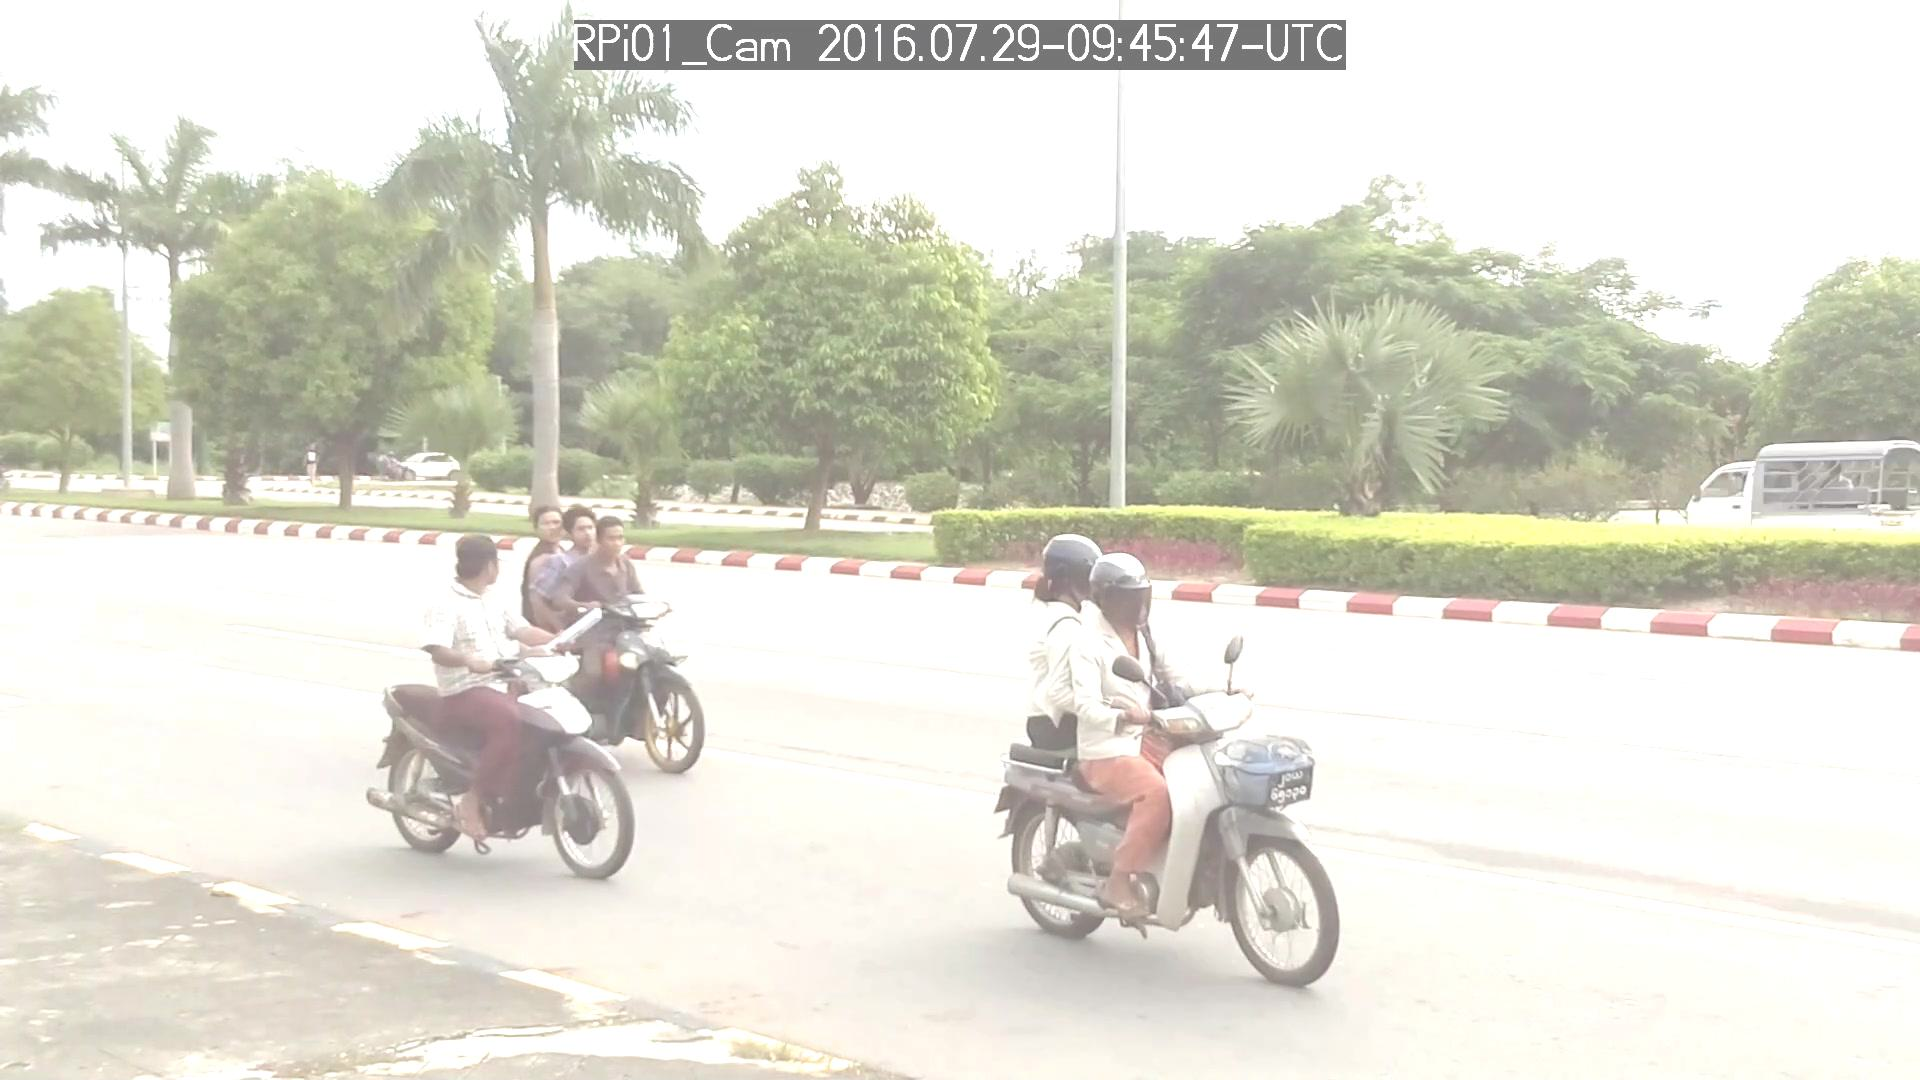
\includegraphics[width=\textwidth]{figs/chap03/rb_origin.jpg}
        \caption{随机亮度}
        \label{fig:sub1}
    \end{subfigure}
    \begin{subfigure}[t]{0.3\textwidth}
        \centering
        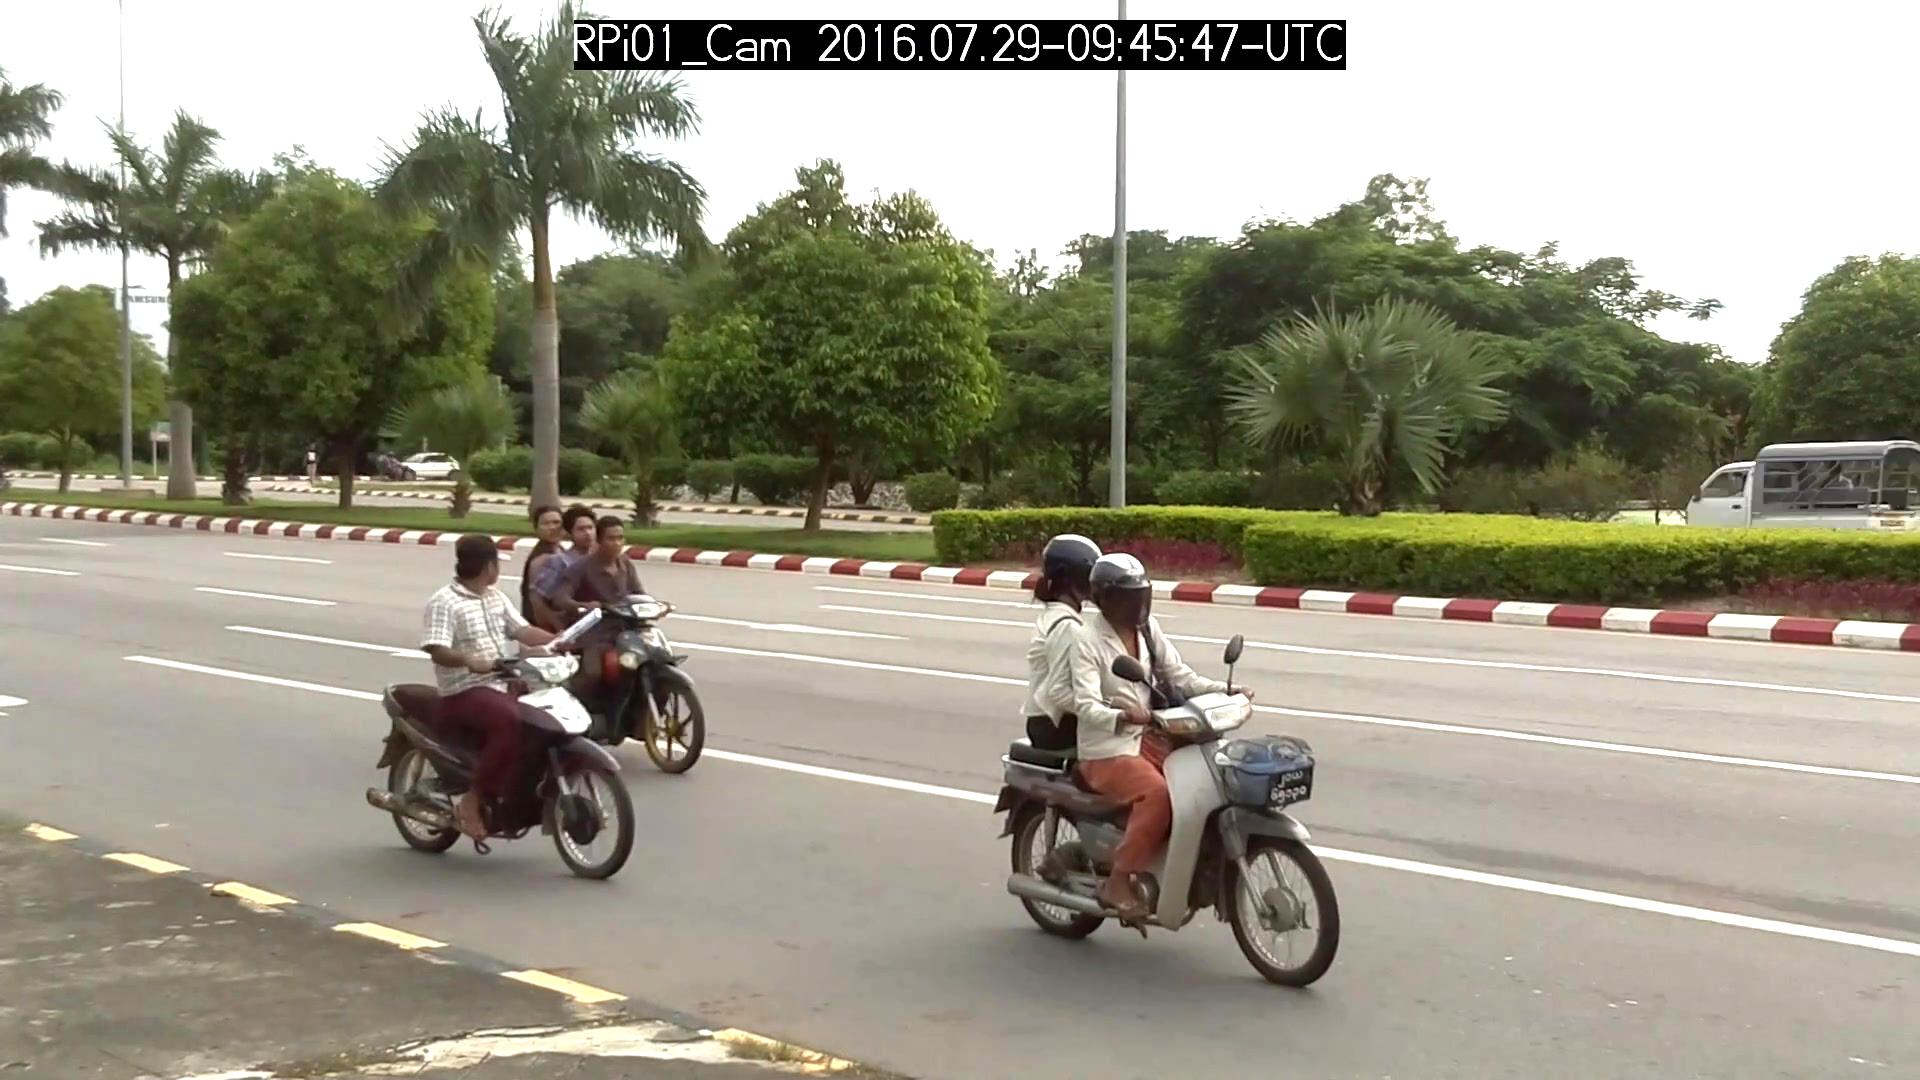
\includegraphics[width=\textwidth]{figs/chap03/rc_origin.jpg}
        \caption{随机对比度}
        \label{fig:sub2}
    \end{subfigure}
    \begin{subfigure}[t]{0.3\textwidth}
        \centering
        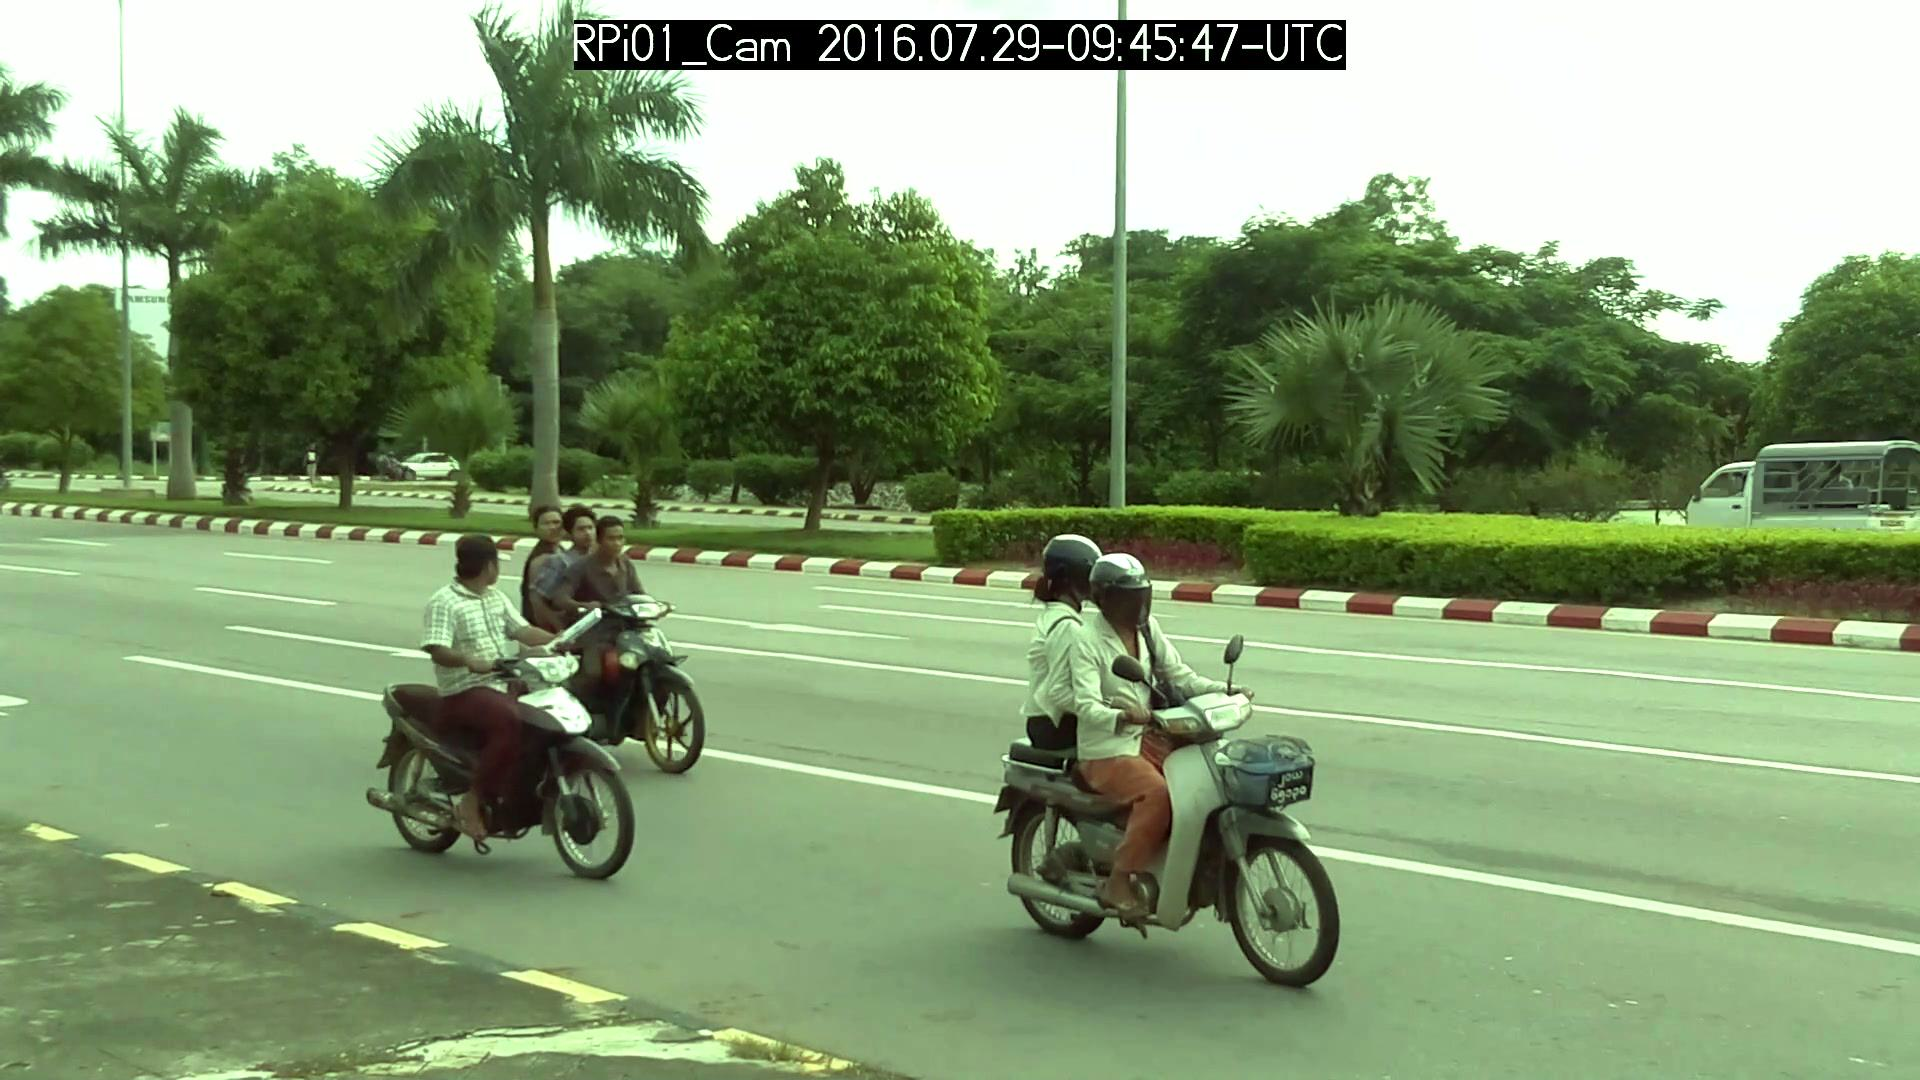
\includegraphics[width=\textwidth]{figs/chap03/rs_origin.jpg}
        \caption{随机饱和度}
        \label{fig:sub3}
    \end{subfigure}

    \begin{subfigure}[t]{0.3\textwidth}
        \centering
        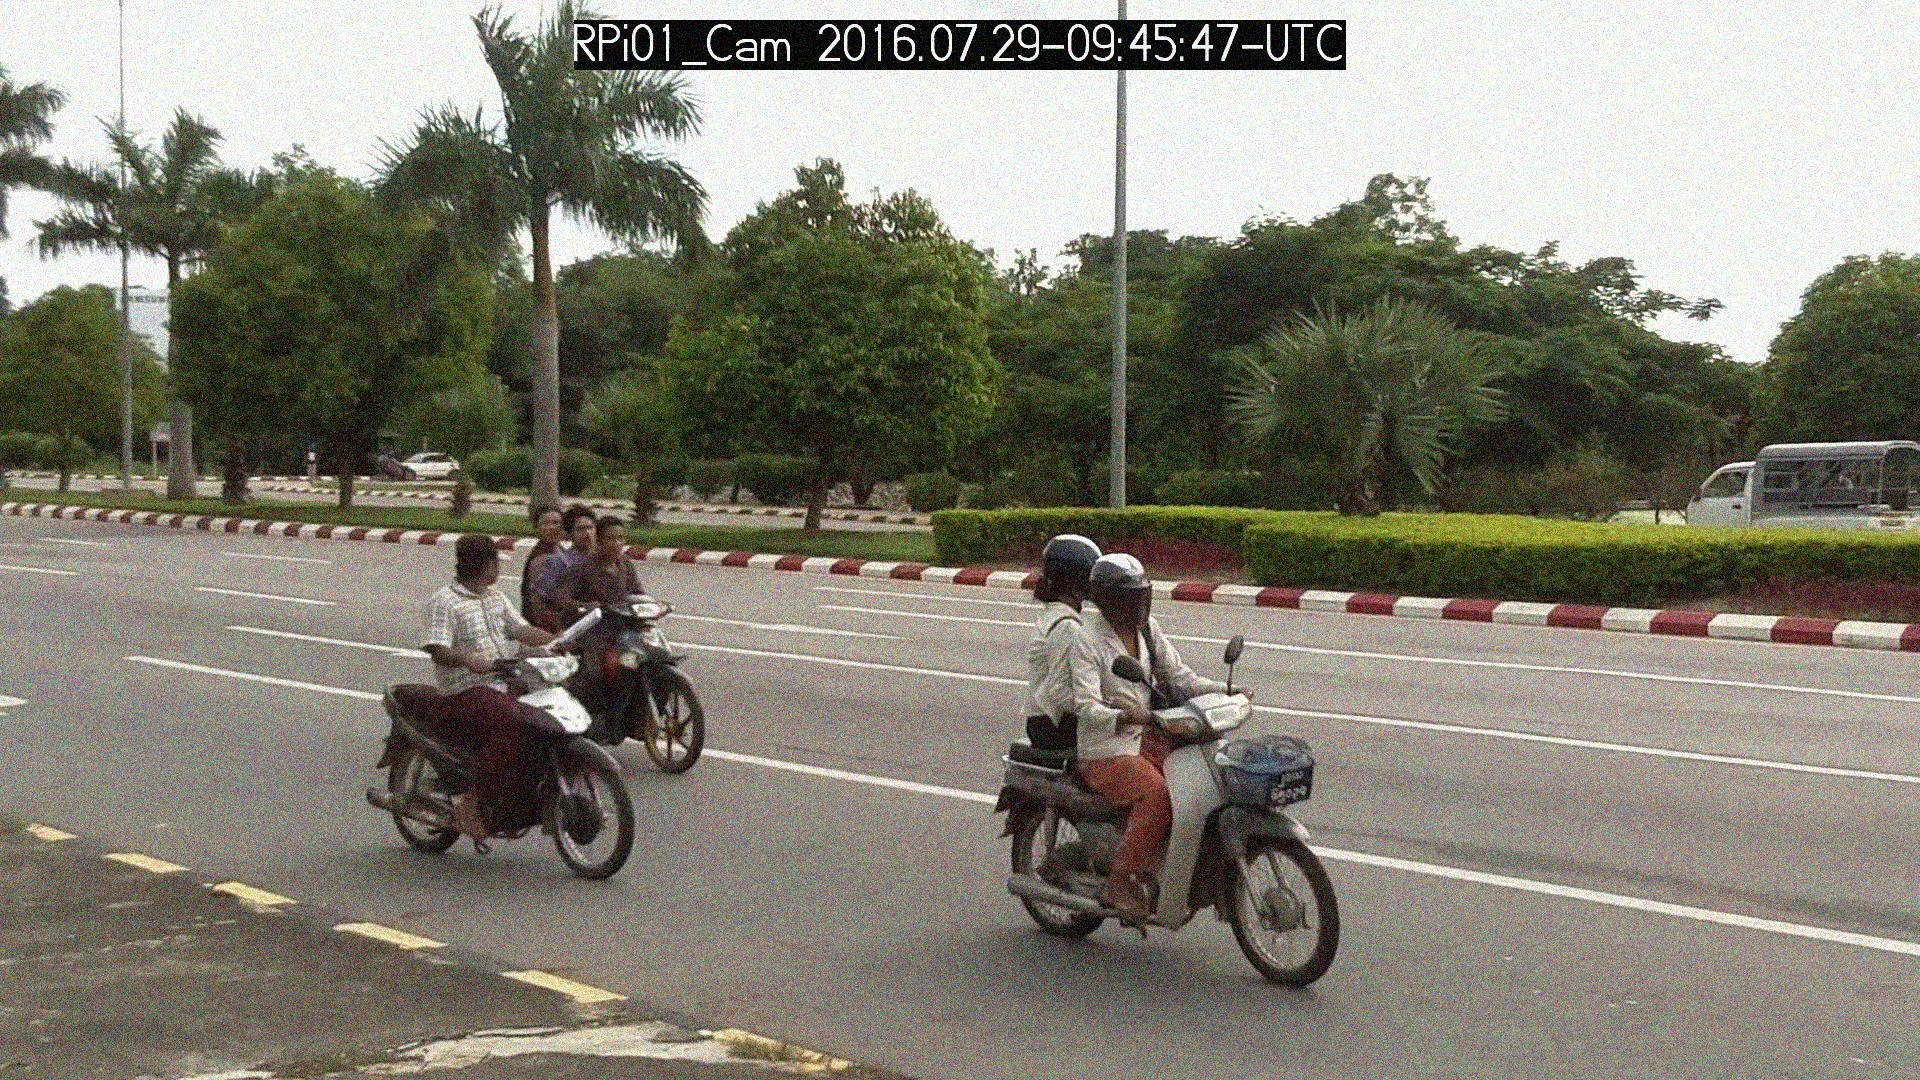
\includegraphics[width=\textwidth]{figs/chap03/gn_origin.jpg}
        \caption{高斯噪声}
        \label{fig:sub4}
    \end{subfigure}
    \begin{subfigure}[t]{0.3\textwidth}
        \centering
        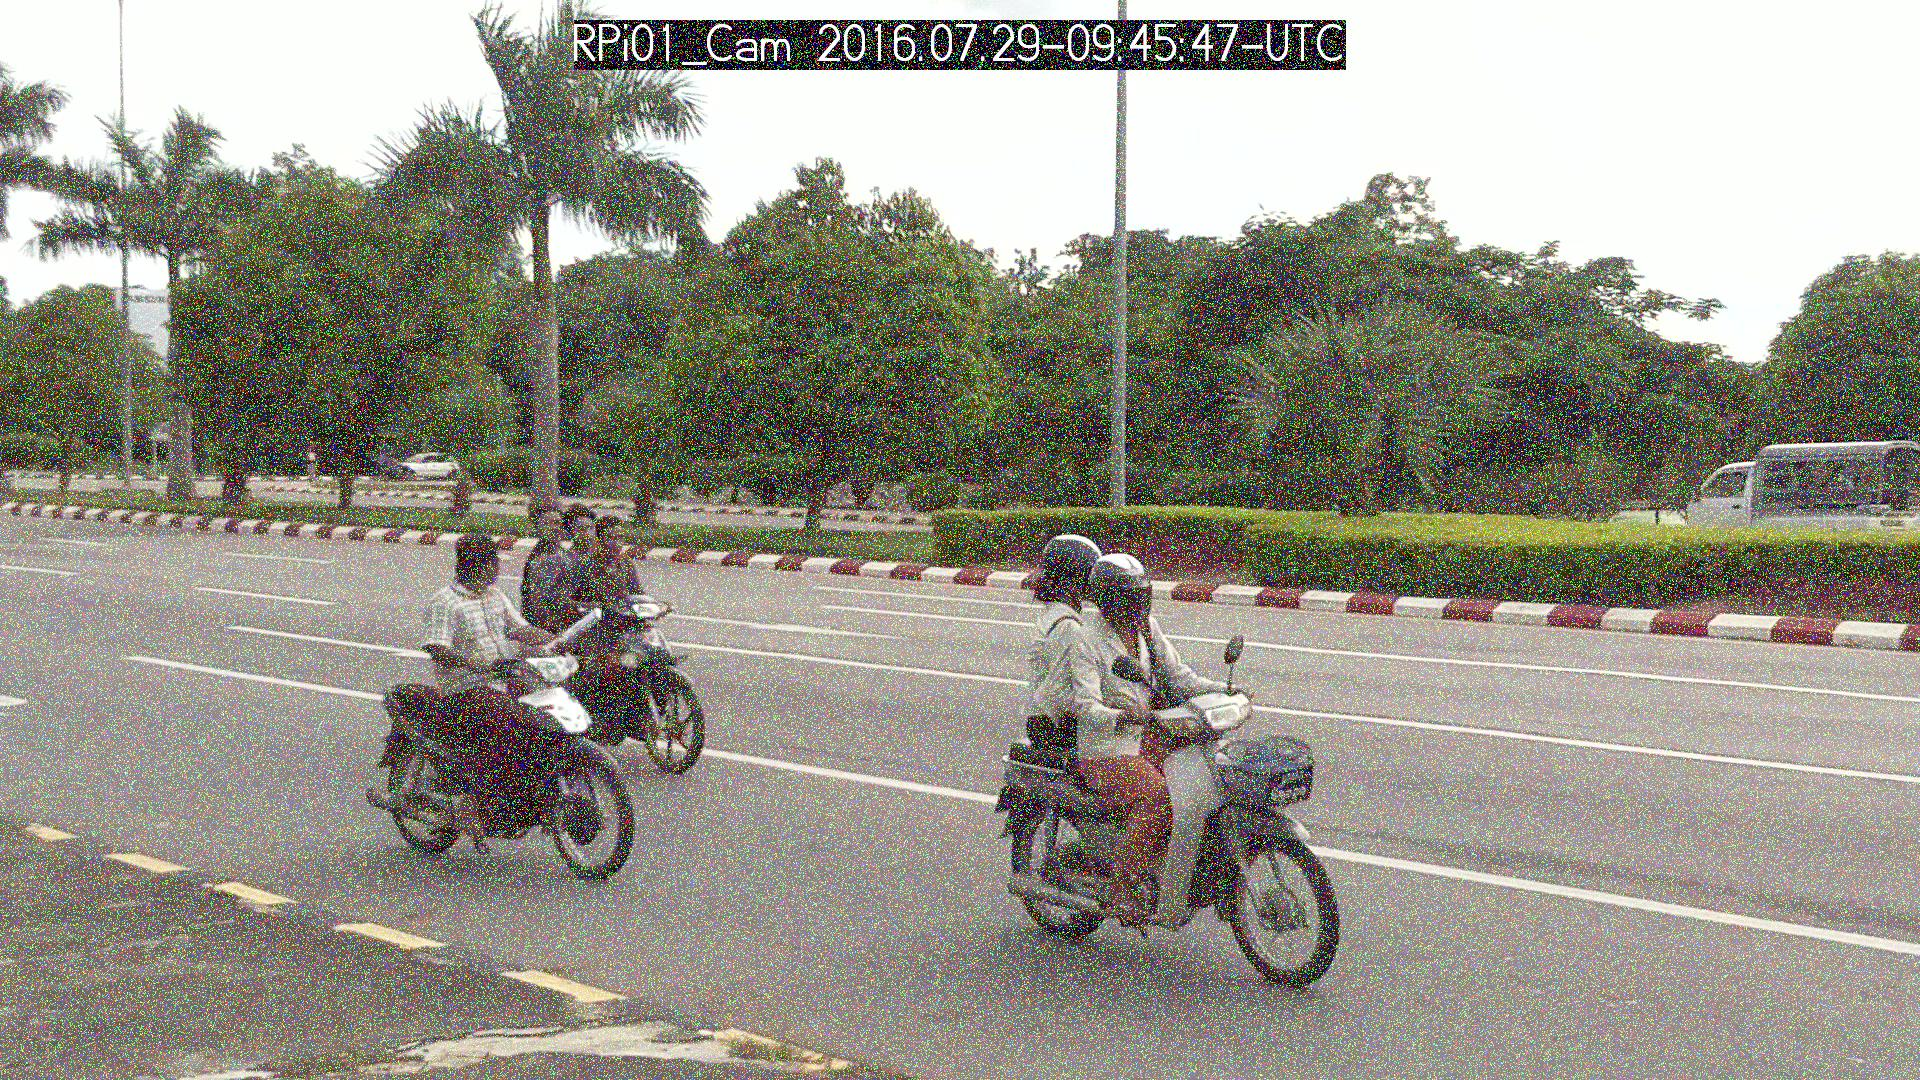
\includegraphics[width=\textwidth]{figs/chap03/sn_origin.jpg}
        \caption{salt噪声}
        \label{fig:sub5}
    \end{subfigure}
    \begin{subfigure}[t]{0.3\textwidth}
        \centering
        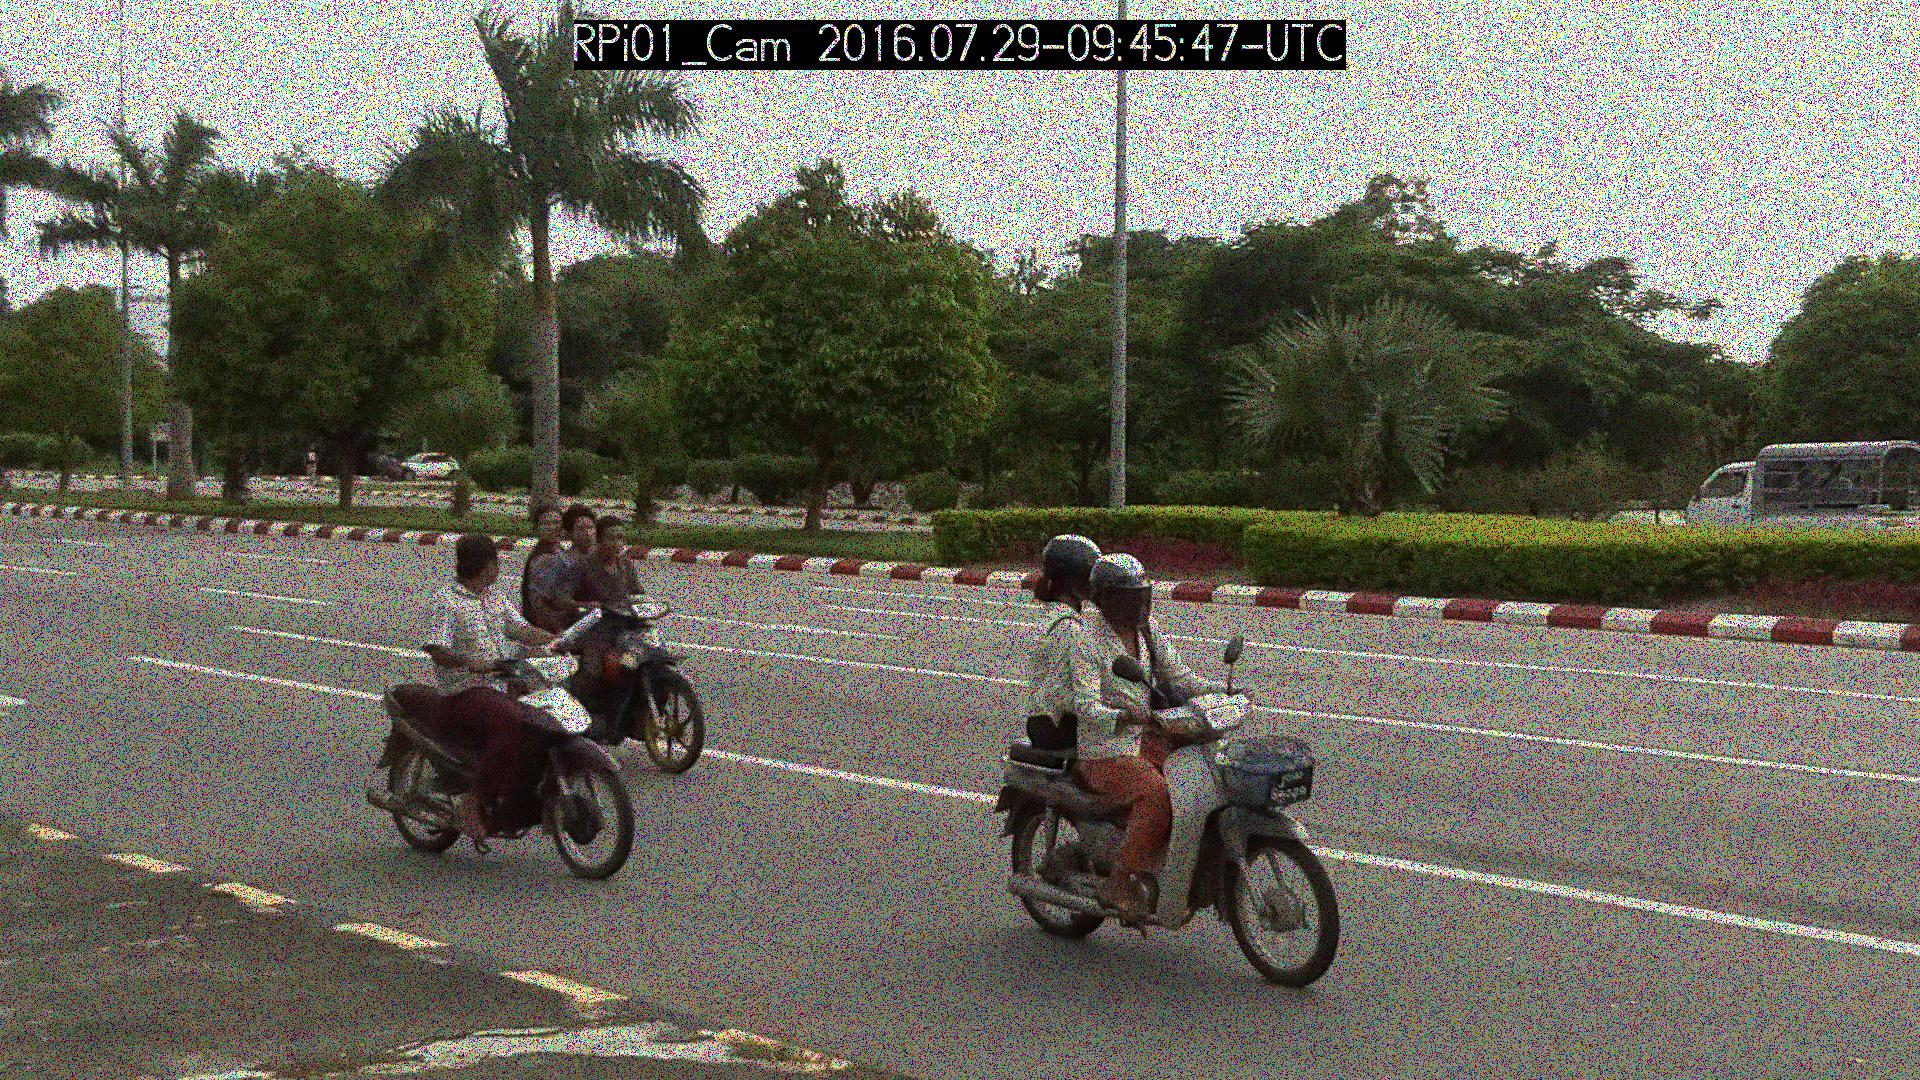
\includegraphics[width=\textwidth]{figs/chap03/pn_origin.jpg}
        \caption{pepper噪声}
        \label{fig:sub6}
    \end{subfigure}
    \caption{图像增强方式}
    \label{fig:enhance}
\end{figure}

对原数据集进行增强之后,共有6282张图片,采用7:2:1的比例对数据集进行随机划分,分别构建训练集、验证集和测试集。本文将目标类别分为18类,标签为S01-S18,其对应关系以及含义如\ref{tab:newlabel}所示,其中meaning一列命名规则为:D(Driver)代表摩托车驾驶员,P(Partner)代表乘车人员。P1代表驾驶员身后的一名乘车人员,P2代表驾驶员身后的另一名乘车人员,P0代表驾驶员身前的乘车人员(在原数据集中,某些小朋友会坐在驾驶员身前)。而D、P0、P1和P2后面紧跟着该乘车人员的头盔佩戴情况,Helmet代表已佩戴头盔,NoHelmet代表未佩戴头盔。例如,标签为S09的含义为DNoHelmetP0NoHelmetP1NoHelmet,表示摩托车驾驶员D未佩戴头盔,驾驶员身前的乘车人员P0未佩戴头盔,驾驶员身后的一名乘车人员P1未佩戴头盔。

\begin{table}[htb]
    \centering
    \caption[标签解释]{目标类别标签含义\label{tab:newlabel}}
    \begin{tabular}{lcl}
        \toprule
        \multicolumn{1}{c}{class} & \multicolumn{1}{c}{label} & \multicolumn{1}{l}{meaning} \\
        \midrule
        0 & S01 & DHelmetP1NoHelmetP2NoHelmet \\
        1 & S02 & DNoHelmetP1NoHelmetP2NoHelmet \\
        2 & S03 & DHelmetP0NoHelmetP1NoHelmet \\
        3 & S04 & DNoHelmetP1NoHelmet \\
        4 & S05 & DHelmetP0NoHelmet \\
        5 & S06 & DNoHelmet \\
        6 & S07 & DNoHelmetP1NoHelmetP2Helmet \\
        7 & S08 & DHelmetP1NoHelmet \\
        8 & S09 & DNoHelmetP0NoHelmetP1NoHelmet \\
        9 & S10 & DNoHelmetP1Helmet \\
        10 & S11 &  DHelmetP0NoHelmetP1Helmet \\
        11 & S12 &  DNoHelmetP0NoHelmetP1NoHelmetP2NoHelmet \\
        12 & S13 &  DHelmetP1NoHelmetP2Helmet \\
        13 & S14 &  DNoHelmetP0NoHelmet \\
        14 & S15 &  DHelmet \\
        15 & S16 &  DHelmetP1Helmet \\
        16 & S17 &  DHelmetP0Helmet \\
        17 & S18 &  DHelmetP1HelmetP2Helmet \\
        \bottomrule
    \end{tabular}
\end{table}

18个类别的样本数量分布如\ref{fig:label1}所示,可以看出S15标签数量最多,共6742个,其表示单一驾驶员佩戴头盔;S06标签数量次之,共6346个,其表示单一驾驶员未佩戴头盔,二者实例数量远高于其他标签。说明单一驾驶员驾驶摩托车是最常出现的情况,且佩戴头盔要比不佩戴头盔的情况稍多一些。除上述两个标签之外,S16和S04是数量最多的两个标签,S16标签共3296个,表示驾驶员和身后的一名乘客都佩戴头盔;S04标签共2503个,表示驾驶员和身后的一名乘客都未佩戴头盔。

由表中数据可以看出,单一驾驶员驾驶摩托车的情况出现次数最多,其次是驾驶员携带一名乘客的情况。并且不管是单一驾驶员,还是驾驶员携带一名乘客,佩戴头盔的情况均多于不佩戴头盔的情况。而一名驾驶员携带一名以上乘客的情况比较少见。

\begin{figure}[!htb]
    \centering
    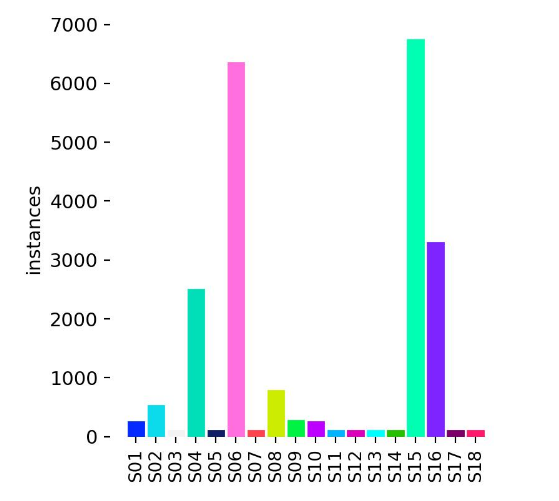
\includegraphics[width=0.8\textwidth]{figs/chap03/label1.png}
    \caption{头盔佩戴情况标签数量分布}
    \label{fig:label1}
\end{figure}

对原数据集5661张图片中的每一个驾驶员目标框进行裁剪,得到33571张包含驾驶员信息的图片,共有570个不同驾驶员。由于驾驶员的图片样本也存在不平衡的情况,对这33571张图片同样进行图像增强,保证每一个驾驶员都至少有100张样本图片。

% \begin{figure}[!htb]
%       \centering
%       \begin{minipage}{0.45\textwidth} % 调整宽度以适应需求,两张图总宽度接近1
%           \centering
%           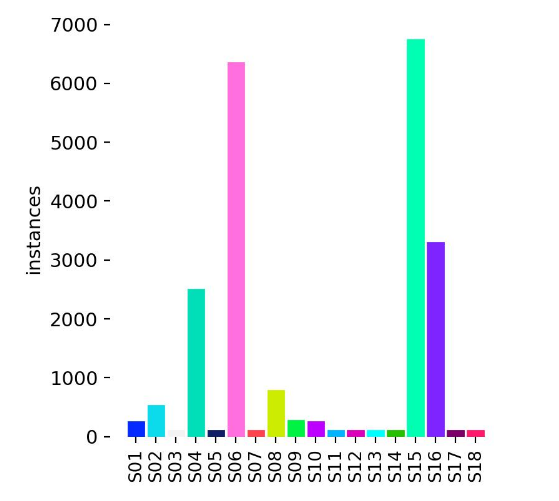
\includegraphics[width=\textwidth]{figs/chap03/label1.png}
%           \caption{头盔佩戴情况标签数量分布}
%           \label{fig:label1}
%       \end{minipage}
%       \hfill % 使两张图片之间保持一定距离
%       \begin{minipage}{0.45\textwidth}
%           \centering
%           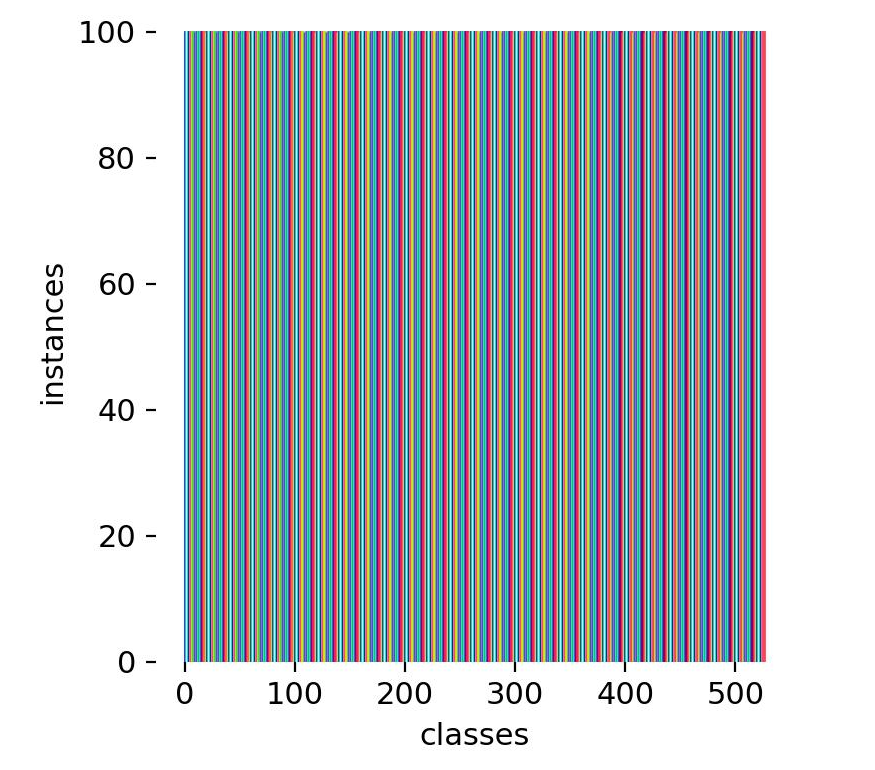
\includegraphics[width=\textwidth]{figs/chap03/label2.png}
%           \caption{驾驶员标签数量分布}
%           \label{fig:label2}
%       \end{minipage}
% \end{figure}

\section{实验环境}
操作系统:Ubuntu 20.04.3 LTS (Focal Fossa)

CPU:Intel(R) Xeon(R) Gold 5318Y CPU @ 2.10GHz

内存:1.5T

GPU:NVIDIA A40

显存:48G

CUDA版本:12.2

Pytorch版本:2.7.0+cu126

\section{参数设置}
本文分别使用YOLOv11n.pt、YOLOv11s.pt、YOLOv11m.pt进行训练,参数设置见\ref{tab:param}。本文进行头盔佩戴情况检测模型训练时,共有18个标签,在yaml文件里nc设置为18。在训练模型中,将batch设置为16,输入图像的size默认设置为640x640,epochs设置为300。
degrees设置为20,在指定度数范围内随机旋转图像,提升模型对摄像头拍摄到的不同角度的图像的识别能力。hsv\_v设置为0.6,将图像的亮度修改一部分,模拟不同的光照环境。translate设置为0.2,将图像进行水平和垂直平移,有助于检测部分可见物体。

\begin{table}[htb]
    \centering
    \caption[标签解释]{参数设置\label{tab:param}}
    \begin{tabular}{lll}
        \toprule
        \multicolumn{1}{l}{param} & \multicolumn{1}{l}{value} & \multicolumn{1}{l}{meaing}\\
        \midrule
        nc & 18 & 类别数量\\
        batch & 16 & 训练批次\\
        size & 640x640 & 输入图像的尺寸\\
        epochs & 300 & 训练轮数\\
        degrees & 20 & 控制图像随机旋转的度数范围\\
        hsv\_v & 0.6 & 控制图像亮度调整幅度\\
        translate & 0.2 & 控制图像在水平和垂直方向上的平移程度\\
        \bottomrule
    \end{tabular}
\end{table}


\section{本章小结}
本章主要介绍了原数据集的来源和本文使用到的六种数据增强方式,展示了需要训练的两个模型的标签及其数量分布。简要介绍了实验环境以及训练的参数设置,说明了本文将基于YOLOv11的三个不同量级的模型进行训练,比较各自的性能。


% % 本文件是示例论文的一部分
% % 论文的主文件位于上级目录的 `main.tex`
% \chapter{数学公式}

% 数学公式是\LaTeX{}排版中举世闻名的强项,关于数学公式的排版。在此,本文无意
% 展开讨论\LaTeX{}中的数学公式排版。只是重点说明一下由 \nwafuthesis{} 提供的
% 特有的宏。

% \section{学习资源}

% 对于数学公式的排版在\enquote{lshort-zh-cn.pdf}的第四章给出了基本的使用方法,
% 请大家阅读学习。其内容对大多数人来说已经足够用了,但是如果不能解决问题的话
% 建议大家求助于搜索引擎或者有经验的人,这也不失为一个好办法。

% 常见的几个学习\LaTeX{}数学公式排版的资源链接如下:

% \begin{itemize}
%   \item 数学排版常见问题集:
%         \url{https://www.latexstudio.net/index/details/index/mid/635}
%   \item \pkg{amsmath}手册中译:
%         \url{https://www.latexstudio.net/index/details/index/mid/706}
%   \item \LaTeX{}公式备忘单:
%         \url{https://www.latexstudio.net/index/details/index/mid/1052.html}
% \end{itemize}

% \section{公式排版与注解}

% 按我校学位论文排版要求,公式排版需要行间居中排版,公式编号按照一级标题(章)
% 连续编号(按章)并加小括号,不加导引线。类似这些细节\nwafuthesis{}模板都已进
% 行了设置。在撰写论文中只要将公式置于\env{equation}环境,并用\cs{label}命令
% 添加标签后用\cs{ref}或\cs{eqref}命令引用该公式即可。对于多行公式可以在
% \env{equation}环境中使用\env{aligned}环境实现排版。

% 需要注意的是,公式解释下面的\enquote{式中}两字需要左起顶格编排,后接符号及
% 其解释;解释顺序为先左后右,先上后下;解释与解释之间用中文分号“;”分隔。
% 此时可以用\cs{noindent}命令临时取消首行缩进,在解释完公式符号后,再次正常
% 用空行进行分段便可自动恢复段落首行缩进。

% 例如:勾股定理可以表示为\ref{eq:gougu}

% \begin{equation}
%   a^2+b^2=c^2\label{eq:gougu}
% \end{equation}

% \noindent
% 式中,$a$是一条直角边边长;$b$是另一条直角边边长;$c$是斜边边长。

% 在公式解释结束后,段落缩进应复位至首行缩进2个汉字的模式。

% \section{模板提供的数学环境}

% \nwafuthesis{} 提供了一系列预定义的数学环境,详情见\nwafuthesis{}说明书的表6。
% 其使用样例有以下7种形式。

% \subsection{axiom公理环境}

% \begin{axiom}[欧几里得距离]
% 点$\mathbf{p}$与点$\mathbf{q}$的\textbf{欧几里德距离},是连接两点的线段
% ($\overline{\mathbf{pq}}$)的长度。

% 在笛卡尔坐标系下,如果 $n$维欧几里得空间下的两个点 $\mathbf{p}=(p_1, p_2,
% \dots, p_n)$ 与点$\mathbf{q} = (q_1, q_2, q_3, \dots, q_n)$,那么点$\mathbf{p}$
% 与点$\mathbf{q}$的距离,或者点$\mathbf{q}$与点$\mathbf{p}$的距离,由
% \autoref{equ:1}定义:
% \begin{align}
% d(\mathbf{p},\mathbf{q}) = d(\mathbf{q},\mathbf{p}) & = \sqrt{(q_1-p_1)^2
%                          + (q_2-p_2)^2 + \cdots + (q_n-p_n)^2} \notag \\
% \label{equ:1}
% & = \sqrt{\sum_{i=1}^n (q_i-p_i)^2}
% \end{align}
% \end{axiom}

% \subsection{corollary推论环境}

% \begin{corollary}[欧几里得距离]
% 点$\mathbf{p}$与点$\mathbf{q}$的\textbf{欧几里德距离},是连接两点的线段
% ($\overline{\mathbf{pq}}$)的长度。

% 在笛卡尔坐标系下,如果 $n$维欧几里得空间下的两个点 $\mathbf{p}=(p_1, p_2,
% \dots, p_n)$ 与点$\mathbf{q} = (q_1, q_2, q_3, \dots, q_n)$,那么点$\mathbf{p}$
% 与点$\mathbf{q}$的距离,或者点$\mathbf{q}$与点$\mathbf{p}$的距离,由
% \autoref{equ:2}定义:
% \begin{align}
% d(\mathbf{p},\mathbf{q}) = d(\mathbf{q},\mathbf{p}) & = \sqrt{(q_1-p_1)^2
%                          + (q_2-p_2)^2 + \cdots + (q_n-p_n)^2} \notag \\
% \label{equ:2}
% & = \sqrt{\sum_{i=1}^n (q_i-p_i)^2}
% \end{align}
% \end{corollary}

% \subsection{definition定义环境}

% \begin{definition}[欧几里得距离]
% 点$\mathbf{p}$与点$\mathbf{q}$的\textbf{欧几里德距离},是连接两点的线段
% ($\overline{\mathbf{pq}}$)的长度。

% 在笛卡尔坐标系下,如果 $n$维欧几里得空间下的两个点 $\mathbf{p}=(p_1, p_2,
% \dots, p_n)$ 与点$\mathbf{q} = (q_1, q_2, q_3, \dots, q_n)$,那么点$\mathbf{p}$
% 与点$\mathbf{q}$的距离,或者点$\mathbf{q}$与点$\mathbf{p}$的距离,由
% \autoref{equ:3}定义:
% \begin{align}
% d(\mathbf{p},\mathbf{q}) = d(\mathbf{q},\mathbf{p}) & = \sqrt{(q_1-p_1)^2
%                          + (q_2-p_2)^2 + \cdots + (q_n-p_n)^2} \notag \\
% \label{equ:3}
% & = \sqrt{\sum_{i=1}^n (q_i-p_i)^2}
% \end{align}
% \end{definition}

% \subsection{example示例环境}

% \begin{example}[欧几里得距离]
% 点$\mathbf{p}$与点$\mathbf{q}$的\textbf{欧几里德距离},是连接两点的线段
% ($\overline{\mathbf{pq}}$)的长度。

% 在笛卡尔坐标系下,如果 $n$维欧几里得空间下的两个点 $\mathbf{p}=(p_1, p_2,
% \dots, p_n)$ 与点$\mathbf{q} = (q_1, q_2, q_3, \dots, q_n)$,那么点$\mathbf{p}$
% 与点$\mathbf{q}$的距离,或者点$\mathbf{q}$与点$\mathbf{p}$的距离,由
% \autoref{equ:4}定义:
% \begin{align}
% d(\mathbf{p},\mathbf{q}) = d(\mathbf{q},\mathbf{p}) & = \sqrt{(q_1-p_1)^2
%                          + (q_2-p_2)^2 + \cdots + (q_n-p_n)^2} \notag \\
% \label{equ:4}
% & = \sqrt{\sum_{i=1}^n (q_i-p_i)^2}
% \end{align}
% \end{example}

% \subsection{lemma引理环境}

% \begin{lemma}[欧几里得距离]
% 点$\mathbf{p}$与点$\mathbf{q}$的\textbf{欧几里德距离},是连接两点的线段
% ($\overline{\mathbf{pq}}$)的长度。

% 在笛卡尔坐标系下,如果 $n$维欧几里得空间下的两个点 $\mathbf{p}=(p_1, p_2,
% \dots, p_n)$ 与点$\mathbf{q} = (q_1, q_2, q_3, \dots, q_n)$,那么点$\mathbf{p}$
% 与点$\mathbf{q}$的距离,或者点$\mathbf{q}$与点$\mathbf{p}$的距离,由
% \autoref{equ:5}定义:
% \begin{align}
% d(\mathbf{p},\mathbf{q}) = d(\mathbf{q},\mathbf{p}) & = \sqrt{(q_1-p_1)^2
%                          + (q_2-p_2)^2 + \cdots + (q_n-p_n)^2} \notag \\
% \label{equ:5}
% & = \sqrt{\sum_{i=1}^n (q_i-p_i)^2}
% \end{align}
% \end{lemma}

% \subsection{proof证明环境}

% \begin{proof}[欧几里得距离]
% 点$\mathbf{p}$与点$\mathbf{q}$的\textbf{欧几里德距离},是连接两点的线段
% ($\overline{\mathbf{pq}}$)的长度。

% 在笛卡尔坐标系下,如果 $n$维欧几里得空间下的两个点 $\mathbf{p}=(p_1, p_2,
% \dots, p_n)$ 与点$\mathbf{q} = (q_1, q_2, q_3, \dots, q_n)$,那么点$\mathbf{p}$
% 与点$\mathbf{q}$的距离,或者点$\mathbf{q}$与点$\mathbf{p}$的距离,由
% \autoref{equ:6}定义:
% \begin{align}
% d(\mathbf{p},\mathbf{q}) = d(\mathbf{q},\mathbf{p}) & = \sqrt{(q_1-p_1)^2
%                          + (q_2-p_2)^2 + \cdots + (q_n-p_n)^2} \notag \\
% \label{equ:6}
% & = \sqrt{\sum_{i=1}^n (q_i-p_i)^2}
% \end{align}
% \end{proof}

% 证明与其他定理环境稍有不同, 末尾会有一个 QED 符号。

% \subsection{theorem定理环境}

% \begin{theorem}[欧几里得距离]
% 点$\mathbf{p}$与点$\mathbf{q}$的\textbf{欧几里德距离},是连接两点的线段
% ($\overline{\mathbf{pq}}$)的长度。

% 在笛卡尔坐标系下,如果 $n$维欧几里得空间下的两个点 $\mathbf{p}=(p_1, p_2,
% \dots, p_n)$ 与点$\mathbf{q} = (q_1, q_2, q_3, \dots, q_n)$,那么点$\mathbf{p}$
% 与点$\mathbf{q}$的距离,或者点$\mathbf{q}$与点$\mathbf{p}$的距离,由
% \autoref{equ:7}定义:
% \begin{align}
% d(\mathbf{p},\mathbf{q}) = d(\mathbf{q},\mathbf{p}) & = \sqrt{(q_1-p_1)^2
%                          + (q_2-p_2)^2 + \cdots + (q_n-p_n)^2} \notag \\
% \label{equ:7}
% & = \sqrt{\sum_{i=1}^n (q_i-p_i)^2}
% \end{align}
% \end{theorem}


% \section{交叉引用}

% 与图表一样,公式、定理等也需要采用专用的命令或环境进行排版以实现
% 编号、交叉引用等\emph{自动化}处理,\emph{万万不可}手动编号、引用!


% %%% Local Variables: 
% %%% mode: latex
% %%% TeX-master: "../main.tex"
% %%% End:
